\documentclass[a4paper, 11pt]{article}

% Language and encoding.
\usepackage[english]{babel}
\usepackage[utf8]{inputenc}

% Set fonts (in order to deal with umlauts).
\usepackage[T1]{fontenc}
\usepackage{lmodern}

% Sets page size and margins.
\usepackage[a4paper, top=2.5cm, bottom=2.5cm, left=3cm, right=3cm, marginparwidth=1.75cm]{geometry}

% Useful packages
\usepackage{graphicx}
\usepackage{subcaption}
\usepackage{url}

% Creative Commons license package.
\usepackage[
    type={CC},
    modifier={by-nc-sa},
    version={4.0},
]{doclicense}

% hyperref package to color links.
%\usepackage[colorlinks=true, allcolors=blue]{hyperref}
\usepackage[hidelinks]{hyperref}

% Todo notes.
%\usepackage[textsize=footnotesize, backgroundcolor=yellow!10, linecolor=gray!35]{todonotes} 

\title{%
	The Gender Gap on Wikipedia \\
	\large{
		Exploring the status quo in research around gender bias related issues
	}
}

\begin{document}

\date{\today}
%\author{E. Jobst and M. Zandpour}
\author{M. Zandpour}
\maketitle

\begin{abstract}
Some abstract...
\end{abstract}

\section{Introduction} \label{sec:intro}
%Gender discrimination is a problem, especially in the technology industry. A recent study~\cite{terrell2017gender} looked at GitHub, one of the most popular software repositories with 14 million users, to see if the effect can be seen by comparing pull requests between male and female contributors. A pull request happens when someone proposes changes on a software code repository that is being hosted on GitHub. The request can either be accepted or denied by the owners of the repository. The researchers found that the approval rates of pull requests, when made without revealing one’s gender, were comparable between both genders~\cite{terrell2017gender}. The rate of approval for women fell significantly if the coder’s gender was identifiable upon requesting a pull whereas the rates for men did not change much~\cite{terrell2017gender}.

Wikipedia, the largest encyclopedia humanity has ever created, has become a critical source of information in our internet driven society. It is entirely crowdsourced. Volunteer editors around the world come together to build out a base of knowledge and make it freely accessible to everyone everywhere. Sometimes, these volunteers are individuals who may have an expertise in a particular subject and share their knowledge freely. But among the people who make contributions to Wikipedia, women pose a serious minority and are disproportionally underrepresented among Wikipedia editors~\cite{shammaa2014}.

Estimations about exact numbers are difficult to find but it is undisputed, that most contributors and even editors are of male gender (see~\autoref{fig:PropFemaleEditors}). The latter is important since editors, specifically veteran editors, do have the powers to reject articles and restrict access of other contributors which has a severe impact on the acceptance rate regarding articles that are written about female figures. The resulting bias with respect to the variety of content is increasingly recognized leading to Wikipedia’s gender gap to be an ever-increasing topic of interest, drawing the attention of scholars of new media and similar fields.

Discussing the systemic bias on Wikipedia is important as the platform poses the most powerful source of information worldwide. It is available in 275 languages and is being accessed by millions of people regularly~\cite{zachte2018}. Many assistive devices and applications such as Smartwatches, Google Assistant, Alexa, Siri or Cortana draw their knowledge directly from Wikipedia without informing their users about the source or authors. Through these developments, the world, as it is represented by Wikipedia, is widely being considered as natural.

In this work, we address gender bias discrepancies within the technology industry by providing an overview over the state-of-the-art in research around the gender gap in open data and open source domains. Additionally, we try to measure possible trends for the future of digital environments that have collaborative characteristics, draw implications for the quality of publicly available information and participation rates and provide suggestions that may have an impact on future developments.

\section{Considerations} \label{sec:considerations}
Most studies on gender bias have been conducted either in Europe or in the United States. Only very few researchers actively work on that topic from other parts of the world. The participants of the studies conducted are more likely to be people from those geographical regions. Thus, their provided data and insights inherently carry strong biases and are not globally representative. A lot of studies in this area are user studies, which poses an issue in our specific case as it can be shown, that women are overall less likely to participate in studies compared to men due to gender-based differences influencing their motivations~\cite{lobato2014impact}. As an example, this phenomenon has an impact on the data used in~\autoref{fig:PropFemaleEditors} since the underlying studies could be skewed accordingly.

\section{Gender Gap on Wikipedia} \label{sec:gender-gap-wikipedia}
In the following we examine several issues connected to Wikipedia’s gender gap and different reasons that are responsible for the low contribution rates of female participants or the low acceptance rate regarding articles about women. We then also make suggestions on how to combat these issues effectively.

\begin{figure}[t]
	\centering
	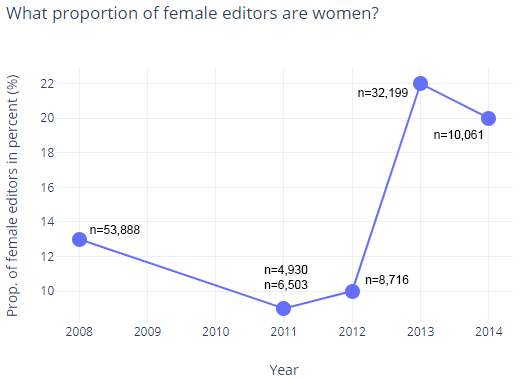
\includegraphics[width=0.85\textwidth]{figures/PropFemaleEditors.png}
\caption{6 Studies were conducted by the Wikimedia Foundation between 2008 and 2014 to measure the proportions between male and female editors that are active on Wikipedia. The specific studies used for this figure can be found in~\autoref{sec:gender-gap-wikipedia:prop-female-editors}.} \label{fig:PropFemaleEditors}
\end{figure}

\subsection{Low proportions of female editors} \label{sec:gender-gap-wikipedia:prop-female-editors}
The Wikimedia Foundation conducts various user studies at annual intervals, and the data thus collected is made publicly available. Part of these studies is also to determine the ratio of female to male editors on Wikipedia. We analyzed the results of the following surveys: Global South User Survey (2014)~\cite{shammaa2014}, Gender micro-survey (2013)~\cite{fung2013}, Editor Survey (2012)~\cite{tilman2012}, Editor Survey (December 2011)~\cite{pande2011}, Editor Survey (April 2011)~\cite{khanna2011}, UNU-MERIT Survey (2008)~\cite{glott2010wikipedia}.

We aimed to see how the ratio of female editors have changed over time. Our results can be seen in~\autoref{fig:PropFemaleEditors}. We found that women are strongly underrepresented within editors on Wikipedia, even in the strongest estimate with 22\% of editors being women in 2013. However, a positive trend can also be observed from the year 2011 onward.

\subsection{Self-perception as a major cause for the gender gap} \label{sec:gender-gap-wikipedia:self-perception}
A characteristic with a particularly strong influence on the interest in participating in the processing of publicly accessible information is self-perception. Hinnosaar et al. showed, that there are significant differences in self-perception and confidence between both genders~\cite{hinnosaar2019gender}. The reason for that is unknown. This difference could be due to women being socialized to be less self-confident or that their experiences lead them to become less self-confident, as the authors note, but this needs to be subject for further studies and investigations as the paper did not aim to find the cause for the discrepancy found. They showed, that the gender gap in Wikipedia editing is, to a large share, because one’s belief about competence~\cite{hinnosaar2019gender}.

These findings are supported by the studies of Collier \& Bear et al.~\cite{collier2012conflict} and Protonotarios \& Sarimpei et al.~\cite{protonotarios2016similar}, but it cannot be shown if the reasons for that lie within the internal structures of Wikipedia, such as sexism within the Wikipedia community, or if these are caused by external factors such as societal standards and expectations.

\subsection{The influence of conflicts on female contributions} \label{sec:gender-gap-wikipedia:conflicts}
Lam \& Uduwage performed a variety of quantitative analyses on publicly available English Wikipedia articles and found, that new users, who could be publicly identified as female, were more likely to stop editing and leave Wikipedia when their edits were reverted~\cite{lam2011wp}. This poses an issue regarding the balance of equal representatives on Wikipedia since the number of female editors attempting to join Wikipedia is already very low.

They also found that articles, where female editors dominated on the amount of contributions, had significantly more disagreements in discussions around edits than other articles~\cite{lam2011wp}. Being subject to large amounts of conflicts causes discomfort and demotivation when it comes to editing other people’s work, since the editors fear to receive even more critical feedback and have their contributions being reverted.

\subsection{Article rejection due to notability criteria} \label{sec:gender-gap-wikipedia:notability}
Wikipedia consists of multiple categories for different types of topics. Although all articles seem to share a similar styling, they belong to different categories. A user can navigate through those categories and see lists of articles belonging to any selected category. For example, there is a category on computer scientists, where a user can find various related lists of scientists such as lists by nationality.

Such categories often have their own communities of editors that are active in the corresponding field who can sometimes impose very harsh acceptance criteria, so that the attempt to publish articles in the respective area often gets rejected due to the lack of fulfillment of said criteria. Wagner et al.~\cite{wagner2016women} found, that there are many areas in Wikipedia where the criteria are unfavorable towards female figures. This is the reason why many articles about women are rejected which further leads to discrepancies when it comes to the ratio of male to female representation regarding Wikipedia articles.

But Klein et al.~\cite{klein2016monitoring} shows that this situation is getting considerably better as societal changes take place with the feminism movement gaining more traction and with public attention being drawn towards a more considerate behavior towards other genders. Initiatives such as meet-ups, talks and competitions with special emphasis on female participants show a net positive development when it comes to public perception and awareness towards women and women’s rights worldwide fostering opportunities for women to overcome societal hurdles and gain equal access to positions within higher ranking institutions and well paid job opportunities. Such societal changes are strongly reflected within Wikipedia as well.

\subsection{Content differences between articles about men and women} \label{sec:gender-gap-wikipedia:contentdiff}
Wikipedia allows to link to other articles in the text of an article. This simplifies explanations of terms and connects coherent, relevant information without packing everything into one page and losing the overview. Wagner et al. found that these internal links within articles about women frequently lead to articles about men while in comparison, men who are interlinked to women very often lack such internal Wikipedia links to the articles of the corresponding women~\cite{wagner2015s}.

This makes it look as if it is women who are usually related to men and not the other way around. Relating to this issue, Graells-Garrido et al. found, that the spouse attribute in articles about women is included significantly more often than in articles about men~\cite{graells2015first}. Recommendation and search algorithms depend on strong connections between Wikipedia articles and the lack of those can lead to women being discriminated when it comes to ranking articles regarding their notability.

Even the language used within articles compared between men and women is different. Wagner et. al and Graells-Garrido et al. both showed that articles about women contain significantly more information about relationship and family issues compared to articles about men~\cite{wagner2015s}~\cite{graells2015first}. This may be due to societal issues such as women often being related to the home domain and relationship domain.

\subsection{How to combat the gender gap on Wikipedia} \label{sec:gender-gap-wikipedia:combatgap}
\subsubsection{Being more considerate towards newcomers} \label{sec:gender-gap-wikipedia:newcomers}
To prevent newcomers from being further scared off because of conflicts, Wikipedia editors must be more careful with their power to discard proposed changes. This aspect should be included in the Wikipedia guidelines and clearly emphasized. Proposed changes of positive intent should be encouraged by giving more thought to thanking users for their contributions.

Such a reaction is also publicly visible and of great interpersonal importance. It can also strengthen the self-esteem of the users concerned, thereby improving the perception of the competence of newcomers. This in turn could be beneficial in terms of motivation to edit existing articles or to create new articles.

\subsubsection{Information events for women} \label{sec:gender-gap-wikipedia:infoevents}
To further battle the gap, increasing efforts need to be put to invite women as contributors on Wikipedia. This can be done through explicit information events that focus on women. There are independent associations around the world that are affiliated with the Wikimedia Foundation and promote Wikipedia's mission to facilitate the distribution of freely available information.

One such organization exists in Vienna, for example, and stages weekly open access information events where anyone can visit their office and learn how to write or edit articles on Wikipedia. Such associations need to put more effort into attracting the attention of women and encouraging their contributions, considering the use of direct and indirect marketing methods with appropriately targeted content. In addition, opportunities could be created for women to socialize with each other.

\subsubsection{Notability criteria} \label{sec:gender-gap-wikipedia:fixnotability}
When it comes to notability criteria, editors need to double check their stance on the importance of such figures. It often happens that women who have made meaningful achievements within their communities and therefore are of great value to recognized groups of people do not receive equal recognition from the Wikipedia community, even though their achievements are often recognized as being important and can be verified by trustworthy primary and secondary literature and other sources. This needs to be discussed and considered by editors of different sections and categories within Wikipedia.

\subsubsection{Historical accuracy} \label{sec:gender-gap-wikipedia:historyaccuracy}
Articles about women, especially historic figures, need to be revised and added. As an example, Wikipedia lacks a lot of data about women from the 1940s to 1950s and existing articles suffer a lot from historic biases since the sources used were already biased. This requires serious investigative efforts to obtaining the facts and curate the information into Wikipedia.

\subsubsection{Language} \label{sec:gender-gap-wikipedia:language}
The social influence of Wikipedia is undisputed. It is important to help raise public awareness and make people sensitive to the various forms of discrimination. This includes discrimination through language, including that used to write or edit articles on Wikipedia. Stereotypes and prejudices are made about women in all areas of life and social environments. This discriminatory use of language takes place in everyday conversations, in the media, in textbooks, on the labor market, etc. and is accepted, used and passed on, consciously or unconsciously, reflected or unreflected~\cite{peters2017bbc}. Correspondingly stereotypical texts also exist in Wikipedia~\cite{graells2015first}.

The starting point for any discrimination is prevailing social norms, which are set by the majority within a society and do not take into account differences. Non-discriminatory language must be perceived and practiced individually in everyday life. Language is often understood as a neutral means of communication, but it is a very powerful tool when it comes to giving meaning and significance to our world. We discriminate against others not only by what we do, but also by what we say and what we don't say. Wikipedia is particularly subject to implicit language discrimination, for example when relevant information is systematically not mentioned or irrelevant, stereotypical information is highlighted~\cite{wagner2016women}.

Some common spelling rules should be considered when writing or editing articles. As an example: women in politics are often described as female politicians, whereas articles about male politicians do not mention gender. This gives the impression that male is the standard gender and that women are "something different" in comparison~\cite{wagner2016women}. When categorizing articles, equal treatment must be ensured, because a similar effect can be caused by, for example, moving female politicians into a separate category called "female politicians" while leaving male politicians in the "politicians" category~\cite{flood2013guardian}. This creates the impression that female politicians need an explicit adjective to distinguish them from politicians in general. This is especially important in the lead part of the article, since most people, as well as software applications, pay most attention to that section.

Likewise, one should avoid using expressions like "She was the first woman to ..." as they put gender above actual achievement and indirectly emphasize that there have been men who have already achieved the same, which could be perceived as reducing the value of the achievement. These formulations can have the effect that the respective woman has succeeded in achieving a less valuable form of said achievement, but is still worthy of attention because of her femininity. Also, family references should be used just as sparingly with women as with men.

The importance of a woman should not be defined exclusively in terms of her relationship with other men. Accordingly, care should be taken to ensure that mentions such as relationship status, marriage, divorce or sexuality are mentioned in a meaningful, context-related way~\cite{graells2015first}. If it is considered appropriate to mention marriage to a man, then expressions such as "man and wife" should be avoided. Instead of "A is the wife of B", "A is married to B" should be used as a form of expression, since otherwise the man is treated in a generalizing manner, but the woman is explicitly marked.

\section{Conclusion} \label{sec:conclusion}

% References section.
\bibliographystyle{plain}
\bibliography{bibliography}

% Add CC license.
\doclicenseThis

\end{document}
